% id: 0270
% book: RPM 중3-2 수학 · 03 원과 직선
% section: 유형 01 현의 수직이등분선 (1)
% figure: crop:fig-0270.png
% answer: $2\sqrt{37}$
% answer_source: 답지
% variant_level: 0 (원본 전사)
% 이 파일은 build.mjs 가 items.json 에서 만든다. 고칠 때는 items.json 을 고친다.
\noindent\begin{minipage}[t]{0.58\linewidth}\vspace{0pt}\raggedright 오른쪽 그림의 원~$\pt{O}$에서 $\seg{AB}\perp\seg{OM}$, $\seg{CD}\perp\seg{ON}$이고 $\seg{AB}=10$, $\seg{OM}=4$, $\seg{ON}=2$일 때, 현~$\pt{CD}$의 길이를 구하시오.\end{minipage}\hfill\begin{minipage}[t]{0.4\linewidth}\vspace{0pt}\centering \setlength{\dmfigw}{61.2pt}\ifdim\dmfigw>\linewidth\setlength{\dmfigw}{\linewidth}\fi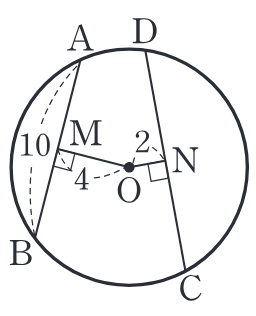
\includegraphics[width=\dmfigw]{figures/fig-0270.png}\end{minipage}\par
